%!TEX root = ../thesis.tex
\chapter{Blockchain}
\label{blockchain}

A blockchain is a distributed transaction ledger~\cite{nakamoto2012bitcoin}. A blockchain consist of a continuously growing list of blocks which are linked, ordered, and immutable. Each block typically contains a hash pointer being a link to a previous block, a timestamp and a list of transactions. Transactions describe transfer of assets from one entity to another. A distributed network is formed by the users of the system, without central control. Each entity of the network contains a local copy of the blockchain; the transaction ledger. To come to an agreement of the correct ledger, the network use a decentralized consensus mechanism with which integrity is achieved and malicious activity is prevented.

Blockchains are potentially suitable for financial activities, the recording of events, medical records~\cite{blockchain_ehr,Azaria2016}, and other records management activities, such as identity management, transaction processing or documenting provenance. Blockchain could be seen as a distributed immutable, tamper-proof, and audit log that records every data transaction. As a result any attempt to tamper blockchain is immediately evident and easily detectable.

Bitcoin~\cite{nakamoto2012bitcoin} is the first decentralized cryptocurrency, a monetary system without central control which solved the double spending problem~\cite{double_spent, nakamoto2012bitcoin}, invented by an unknown person or group of people under the name Satoshi Nakamoto~\cite{nakamoto2012bitcoin}.

The goal of this chapter is the presentation of the basic operating principles of the blockchain, which are based on the foundation of cryptography, without getting to unnecessary details or rigorous mathematical proofs. As Bitcoin was the first decentralized blockchain system and put the bases for other blockchain systems to be made and involve, we mostly focus on its blockchain structure. Notable variations of succeeded blockchains are mentioned selectively.

\section{History}\label{blockchain:history}

Credit card transactions are the dominant payment method that is used on the web today~\cite{Narayanan:2016:BCT:2994437} handled by a financial
system involving processors, banks, credit card companies and other intermediaries. Normally, a credit card transaction is done as follow:
the buyer sends over his credit card details to the merchant, and then the merchant sends and validates the data in the financial system.

Buyers may feel uncomfortable to handle their credit card details to an unknown vendor without good reputation, especially over an insecure channel.
Intermediate services, such as Paypal, sits between the buyer and the seller and the intermediate service has the buyer's credit card details which approves
the transaction and notify the seller. Through this architecture the buyer is not exposed to security risks and can be anonymous improving privacy. On the other hand,
both the buyer and the seller might have an account to the same service.

A notable intermediate architecture called SET (Secure Electronic Transaction)~\cite{set} established in 1996 by VISA and MasterCard which goal was to combine the card associations' similar but incompatible protocols. SET allowed parties to identity themselves with the use of
certificates avoiding that way the need of having to enrol with the intermediary. SET failed to gain attraction in the market and the fundamental problem has to do with the end-user certificates issue complexity.

David Chaum is the inventor of the secure digital cash idea which first introduced in his 1983 paper~\cite{Chaum1983}. In 1990 proposed the first off-line e-cash system~\cite{Chaum:1988:UEC:646753.704915} and founded DigiCash~\cite{chaum1983blind}, an electronic money corporation,
which in 1994 sent the first electronic payment.

Digital cash shemes have a potential flaw called double-spending~\cite{10.1007/978-3-662-46803-6_10, 7163021} in which the same digital token can be spent more than once.
Chaum find a way to both keep the system anonymous and prevent double-spending with the use of blind signatures~\cite{Chaum1983,Chaum:1988:UEC:646753.704915}.
Nevertheless, Chauma's solution needed a centralized trusted oracle that validates the transactions. Many cryptographers tried to improve Chaum's et al. scheme such as Okamoto and Ohta~\cite{Watanabe1996} who implemented the subdivisions of coins with the use of Merkle trees~\cite{merkle_tree}.

About the same time, a group of cryptographers called Cypherpunks~\cite{cypherpunk,cypherpunks_manifesto} was formed who advocate the widespread
use of strong cryptography and privacy-enhancing technologies~\cite{cypherpunks_manifesto} as a route to social and political change. Cypherpunks electronic mailing list,
through which they communicating originally, was the predecessor to the mailing list where Satoshi Nakamoto would announce later Bitcoin~\cite{nakamoto2012bitcoin}.

It is worth mentioning that Chaum's ideas have been described as the technical roots of the vision of the Cypherpunks movement~\cite{cypherpunk}.

Chaum patented the blind-signature scheme preventing others from developing ecash system that use the same protocol. As a respond,
Cypherpunks implemented an e-cash system called Magic Money~\cite{magic_money} which violated Chaum's patents.

At the end, DigiCash failed to gain attraction and the main problem was that it was cantered on the user-merchant transaction hence
DigiCash had to persuade banks and merchants to adopt it.

At 1991, Haber et al. proposed a scheme for secure timestamping of digital documents using digital signatures and hash pointers to previous documents
creating a chain of documents' certificates~\cite{Haber1991}. Later, they proposed an improvement in which the documents are collected into a block and
the blocks are linked together in a chain instead of the documents. This data stracture forms the skeleton of Bitcoin's blockchain.

At 1992 cryptographers Dwork and Naor proposed solutions to computational puzzles as a potentional solution to email spam~\cite{Dwork1993},
creating the idea of Proof-of-Work. Later, at 1997, Adam Back proposed a similar idea called Hashcash~\cite{hash_cash}.
A similar Proof-of-Work system as Hashcash is used in Bitcoin for its consensus mechanism.

Wei Dai at 1998 created b-money~\cite{b_money}, an anonymous distributed electronic cash system, in which everyone
could create money using a Proof-of-Work mechanism like hashcash. B-money used the notion of a secured timestamp ledger as used by Haber et al. for digital documents.

Bitcoin was invented by Satoshi Nakamoto in 2008 where he published a paper with the title ``Bitcoin: A Peer-to-Peer Electronic Cash System'' on The Cryptography Mailing list at metzdowd.com~\cite{satoshi_mailing_list} describing the Bitcoin protocol. The Bitcoin network came into existence on 3 January 2009 with the release of the first Bitcoin client, \verb|wxBitcoin|, and the issuance of the first Bitcoins~\cite{btc_client, btc_first_block}. Bitcoin represents the culmination of decades of research in cryptography~\cite{antonopoulos2014mastering} and combines several prior inventions such as b-money and HashCash~\cite{antonopoulos2014mastering}. Bitcoin is the first decentralized electronic cash system that does not relies on a central authority and
provided for the first time a practical solution to the Byzantine Generals' Problem~\cite{byzantine_fault_tolerance} with the use of a consensus mechanism
based on Proof-of-Work which can be used to achieve consensus on decentralized networks for elections, lotteries, assets registries and more~\cite{antonopoulos2014mastering}. As of April 2018, it is the most widely used alternative currency~\cite{10.1007/978-3-642-39884-1_2} with a total market cap around 116 billion US dollars~\cite{btc_cap}.

\section{Identity}\label{blockchain:identity}

In Bitcoin, and in most cryptocurrencies, there is no inherent notion of identities or individual accounts which ``own'' bitcoins~\cite{7163021,nakamoto2012bitcoin}. There is no users, account balance or identities—these all exist only to the extent that they can be imputed from the list of published transactions~\cite{7163021,nakamoto2012bitcoin}.

Identity is defined as a cryptographic key pair $(s_k, p_k)$, where $s_k$ is the private key and $p_k$ the public key. The private key is used for spending ``coin'' and the public key as the address of the user. No real-world name or identifying information are required~\cite{7163021,nakamoto2012bitcoin}.

In Bitcoin, due to the public nature of the blockchain it is sometimes possible to trace the flow of money between public keys (addresses) and conclude that they are likely controlled by the same
individual~\cite{7163021,10.1007/978-3-319-17016-9_1}. For that reason, Bitcoin's identity system is considered pseudonymous. The underlaying non-anonymous Internet infrastructure (nodes leak their IP address when broadcasting transactions),
together with the availability of all bitcoin transactions in the blockchain, has proven to be an anonymity threat~\cite{10.1007/978-3-319-17016-9_1, 7163021,Meiklejohn:2013:FBC:2504730.2504747,6113303,10.1007/978-3-642-39884-1_2,fi5020237}.
Although Bitcoin provides a limited form of unlinkability by letting users create new addresses at any time for any transaction, various techniques, such as transaction graph analysis, can be utilized by an adversary to link together different addresses controlled
by the same entity leading to deanonimity~\cite{7163021,Meiklejohn:2013:FBC:2504730.2504747,6113303,10.1007/978-3-642-39884-1_2,fi5020237}. Furthermore, Bitcoin does not provide untraceability---for each incoming transaction all possible senders are probable---since all transactions are public~\cite{cryptonote}.

Altcoins such as Zerocash~\cite{zcash} and CryptoNote~\cite{cryptonote} were focused on improving bitcoin anonymity and integrated unlinkability to their currency proposals.
In particular, Zerocash utilize zero-knowledge proofs (zkSNARKs~\cite{10.1007/978-3-642-40084-1_6}) which reveal no information at all about the amount or recipients enabling a completely untraceable ledger. On the other hand, CryptoNote uses ring signatures creating a mixing protocol satisfying both untraceability and unlinkability. CryptoNote compared to Zerocash has better performance but weaker anonymity~\cite{7163021}.

\section{Network}\label{blockchain:network}

\section{Structure}\label{blockchain:structure}

The first blockchain was conceptualised and implemented as a core component of Bitcoin which serves as the public ledger for all transactions. The bitcoin design has been the inspiration for other applications~\cite{7163021,10.1007/978-3-662-46803-6_10, ethereum_whitepaper}. In the next subsections we analyze the Bitcoin's blockchain structure.

\subsection{Transactions}\label{blockchain:structure:tx}

The basic data structure of the blockchain is a \textbf{transaction (tx)} that transfers assets from one party to another. The owner of a coin transfers coins by publishing a digital signed statement; his desire to perform a transaction that transfers coins to the recipient of the money. By verifying the signature, one can ensure that the sender of the money is truly the one who authorized the transaction. A blockchain transaction can be described as a node with two edges, one incoming edge and one outcoming edge~\cite{zindros_thesis}. The incoming edge describes the sender (from) and the outcoming edge the recipient (to). Each edge has the corresponding address of the party; her public key. Every bitcoin transaction has a unique \textbf{transaction id (txid)} which is derived by double hashing the whole transaction with the use of the SHA-256 cryptographic hash function. Payments are done thought linking transaction nodes and money can be view as a chain of transactions where monetary value flows~\cite{zindros_thesis}. All transactions together form a transaction graph which is public and everyone participating in the network can see and add new transactions to the graph.

\begin{figure}[!ht]
  \centering
  \begin{subfigure}[!ht]{\textwidth}
    \centering
    \begin{tikzpicture}
      \node[tx] (A) at (0,0) {$tx$};
      \draw [->] ++(-3,0) -- (A) node[midway, below]{Alice} node[midway, above]{5mBTC};
      \draw [->] (A) -- ++(3, 0) node[midway, below]{Bob} node[midway, above]{5mBTC};
    \end{tikzpicture}
    \caption{Simplified}
    \label{fig:bl_tx:simple}
    \vspace*{2mm}
  \end{subfigure}
  \begin{subfigure}[!ht]{\textwidth}
    \centering
    \begin{tikzpicture}
      \node[tx] (A) at (0,0) {$tx$};
      \draw [->] (-3,0) -- (A) node[below, xshift=-4.7cm]{\footnotesize{1BvBMSEYstWetqTFn5Au4m4GFg7xJaNVN2}} node[midway, above]{5mBTC};
      \draw [->] (A) -- (3, 0) node[left, below, xshift=1.5cm]{\footnotesize{1J98t1WpEZ73CNmQviecrnyiWrnqRhWNLy}} node[midway, above]{5mBTC};
    \end{tikzpicture}
    \caption{Addresses are public keys}
    \label{fig:bl_tx:pub}
    \vspace*{2mm}
  \end{subfigure}
  \caption{A bitcoin transaction}
  \label{fig:bl_tx:tx}
\end{figure}

\begin{figure}[!ht]
  \centering
  \begin{tikzpicture}
    \node[tx] (A) at (0,0) {$tx$};
    \draw [->] (-3,0) -- (A) node[midway, below]{Alice} node[midway, above]{5mBTC};
    \draw [->] (A) -- (3, 0) node[midway, below]{Bob} node[midway, above]{5mBTC};
    \node (txid) at (-5,0) {$txid = SHA256^{2}($};
    \node (txid) at (3.3,0) {$)$};
  \end{tikzpicture}
  \caption{Bitcoin Transaction ID}
  \label{fig:bl_tx:id}
\end{figure}

A mechanism is needed to keep track the total money each user has. Otherwise, anyone could produce money arbitrarily, sign it and create a valid transaction. When a transaction is made, each node on the network should be able to confirm that the user making the transaction, has indeed the money to transfer. As there is no central trusted third party, the whole network have to maintain exactly who has how much coin.

Transaction can have outgoing unlinked edges, edges that are not connected to another node transaction. These edges are unspent coins, owned by various users and ready to be spent. This type of edges are called \textbf{unspent transaction outputs (UTXO)}. The UTXO set, the list of all outgoing unlinked edges, describes how much each user owns and is kept from every node of the network. In this way, the recipient and the network can confirm, by checking the UTXO set, that the sender owns the money at the time of the transaction.

When a user wants to transfer money, first she have to find a transaction that has a UTXO of which she is the owner. Then she creates one transaction with one incoming and one outgoing edge and connect the incoming edge of the new transaction with the old UTXO. Now the old UTXO is not an UTXO anymore, it is just spent, and the outgoing edge of the new transaction is unconnected and becomes the new UTXO. Finally she specifies the value and the owner (address) of the new outgoing edge and signs the transaction. The sign of the transaction is a way of declaring asset ownership. The user have to prove that for a public key---the address where the UTXO points to---she holds the corresponding private key. Only the owner of the private key can produce valid signatures that are verifiable under the corresponding public key.

The UTXO set is maintained collectively by the network. When a new full node is connected to the network, the nodes with which it connects inform it about UTXO set and the history of all transactions that occurred from the begging of time. If a full node reconnects after a period on inactivity the node is informed about the new transactions that took place since the last time the node was connected to the network. For the nodes to be able to maintain the UTXO set, the transactions have to be published on the network. This is achieved through a mechanism called broadcasting. When a transaction is created, the participants broadcast the details of the transaction to their neighbours. The neighbours publish the transaction to their neighbours and recursively the transaction is being published until the whole network becomes aware of it.

In Bitcoin there is no notion of giving changes. That is, because there is no accounts with balances and the only way of keeping track money ownership is the UTXO set, the total value of the income edge must be consumed at once. However, a bitcoin transaction can have multiple incoming and outcoming edges. This property is exploited to create a changing system. In particular, when a user wants to transfer money to another user and the value of the UTXO edge is bigger than the desired amount, she can create a transaction with two outcoming edges, one for the recipient and one to give changes to herself.

\begin{figure}[!ht]
  \centering
  \begin{tikzpicture}
    \node[tx] (A) at (0,0) {$tx$};
    \draw [->] (-3,0) -- (A) node[midway, below]{Alice} node[midway, above]{1mBTC};
    \draw [->] (A) -- ++(2, 0) -- ++(1, 1) -- ++(2, 0) node[midway, below]{Bob} node[midway, above]{0.1mBTC};
    \draw [->] (A) -- ++(2, 0) -- ++(1, -1) -- ++(2, 0) node[midway, below]{Alice} node[midway, above]{0.9mBTC};
  \end{tikzpicture}
  \caption{Change exchange}
  \label{fig:bl_tx:change}
\end{figure}

\begin{figure}[!ht]
  \centering
  \begin{tikzpicture}[node distance=3cm]
    \node[tx] (A) at (0,0) {$tx$};
    \node[tx, below of=A] (B) {$tx$};
    \node[tx, below of=B] (C) {$tx$};
    \node[tx, right of=B, node distance=7cm] (D) {$tx$};

    \draw [->] (A) -- ++(4, 0) node[midway, below]{Alice} node[midway, above]{1mBTC} -- (D);
    \draw [->] (B) -- ++(4, 0) node[midway, below]{Alice} node[midway, above]{2mBTC} -- (D);
    \draw [->] (C) -- ++(4, 0) node[midway, below]{Alice} node[midway, above]{1.5mBTC} -- (D);

    \draw [->] (D) -- ++(4, 0) node[midway, below]{Bob} node[midway, above]{4.5mBTC};

  \end{tikzpicture}
  \caption{Transaction multiple inputs}
  \label{fig:bl_tx:change}
\end{figure}

\begin{figure}[!ht]
  \centering
  \begin{tikzpicture}
    \node[tx] (A) at (-5,0) {$tx$};
    \node[tx] (B) at (0,0) {$tx$};
    \draw [->] (A) -- (B) node[midway, below]{Wage} node[midway, above]{1mBTC};
    \draw [->] (B) -- ++(2, 0) -- ++(1, 2) -- ++(2, 0) node[midway, below]{Rent} node[midway, above]{0.6mBTC};
    \draw [->] (B) -- ++(2, 0) -- ++(3, 0) node[midway, below, xshift=1em]{Electricity} node[midway, above, xshift=1em]{0.2mBTC};
    \draw [->] (B) -- ++(2, 0) -- ++(1, -2) -- ++(2, 0) node[midway, below]{Gas} node[midway, above]{0.2mBTC};
  \end{tikzpicture}
  \caption{Transaction multiple outputs}
  \label{fig:bl_tx:multi_out}
\end{figure}

In the Bitcoin transaction graph, the Kirchhoff property mandates that the total outputs of all transactions are at most equal to the total inputs of all transactions. In particular, let $txs$ be all transactions of the network, $out(tx)$ all the output edges of transaction $tx$, $in(tx)$ all the input edges of transaction $tx$ and $w(e)$ the value of that edge, it holds that:

\begin{equation*}
  \forall tx \in txs: \sum_{o \in out(tx)}w(o) \leq \sum_{i \in in(tx)}w(i)
\end{equation*}

\begin{figure}[ht!]
    \centering
    \begin{tikzpicture}[scale=0.9]
      \node[tx] (A) at (0,0) {$tx$};
      \node[tx] (B) at (4,0) {$tx$};
      \node[tx] (C) at (8,0) {$tx$};
      \draw [->] (-3,0) -- (A) node[midway, below]{Alice} node[midway, above]{1mBTC};
      \draw [->] (A) -- (B) node[midway, below]{Bob} node[midway, above]{1mBTC};
      \draw [->] (B) -- (C) node[midway, below]{Charlie} node[midway, above]{1mBTC};
      \draw [->] (C) -- (11,0) node[midway, below]{Eve} node[midway, above]{1mBTC};

      \node[red] (D) at (10, 3) {$utxo$};
      \draw [->, red] (D) -- (10,0.8);
      \node[ellipse, draw, red, inner xsep=4.5ex,inner ysep=1.9ex] at (10,0) {};
    \end{tikzpicture}
  \caption{Transaction graph and UTXO}
  \label{fig:bl_utxo}
\end{figure}

\begin{figure}[ht!]
  \begin{subfigure}[t]{0.50\textwidth}
    \centering
    \begin{tikzpicture}
      \node[tx] (A) at (0,0) {$tx$};
      \draw [->] (A) -- (3,0) node[midway, below]{Alice} node[midway, above]{1mBTC};

      \node[red] (utxo) at (2, 3) {$utxo$};
      \draw [->, red] (utxo) -- (2,0.8);
      \node[ellipse, draw, red, inner xsep=4.5ex,inner ysep=1.9ex] at (2,0) {};
    \end{tikzpicture}
    \caption{Alice finds one UTXO that belongs to her}
    \label{fig:bl_spent:a}
  \end{subfigure}
  \begin{subfigure}[t]{0.50\textwidth}
    \centering
    \begin{tikzpicture}[scale=0.9]
      \node[tx] (A) at (0,0) {$tx$};
      \draw [->] (A) -- (3,0) node[midway, below]{Alice} node[midway, above]{1mBTC};
      \node[tx] (B) at (5,0) {$tx$};
      \draw [->] (B) -- (8,0) node[midway, below]{Bob} node[midway, above]{1mBTC};

      \node[red] (utxo) at (2, 3) {$utxo$};
      \draw [->, red] (utxo) -- (2,0.8);
      \node[ellipse, draw, red, inner xsep=4.5ex,inner ysep=1.9ex] at (2,0) {};
    \end{tikzpicture}
    \caption{Alice create a transaction with recipient Bob}
    \label{fig:bl_spent:b}
  \end{subfigure}
  \begin{subfigure}[t]{0.50\textwidth}
    \centering
    \begin{tikzpicture}[scale=0.9]
      \node[tx] (A) at (0,0) {$tx$};
      \node[tx] (B) at (4,0) {$tx$};
      \draw [->] (A) -- (B) node[midway, below]{Alice} node[midway, above]{1mBTC};
      \draw [->] (B) -- (7,0) node[midway, below]{Bob} node[midway, above]{1mBTC};

      \node[red] (utxo) at (2, 3) {$not\text{ }utxo\text{ }anymore$};
      \draw [->, red] (utxo) -- (2,0.8);
      \node[ellipse, draw, red, inner xsep=4.5ex,inner ysep=1.9ex] at (2,0) {};

      \node[blue] (utxo) at (6, 3) {$new\text{ }utxo$};
      \draw [->, blue] (utxo) -- (6,0.8);
      \node[ellipse, draw, blue, inner xsep=4.5ex,inner ysep=1.9ex] at (6,0) {};
    \end{tikzpicture}
    \caption{Alice connects the incoming edge of the new transaction with the old UTXO}
    \label{fig:bl_spent:c}
  \end{subfigure}
  \begin{subfigure}[t]{0.50\textwidth}
    \centering
    \begin{tikzpicture}[scale=0.9]
      \node[tx] (A) at (0,0) {$tx$};
      \node[tx] (B) at (4,0) {$tx$};
      \draw [->] (A) -- (B) node[midway, below]{Alice} node[midway, above]{1mBTC};
      \draw [->] (B) -- (7,0) node[midway, below]{Bob} node[midway, above]{1mBTC};

      \node[red] (utxo) at (4.8, 3) {$Alice\text{ }signs\text{ }$};
      \node[ellipse, draw, red, inner xsep=8ex,inner ysep=4ex] (ell) at (4.8,0) {};
      \draw [->, red] (utxo) -- (ell);
    \end{tikzpicture}
    \caption{Alice signs the transaction. No one else can forge this signature}
    \label{fig:bl_spent:d}
  \end{subfigure}
  \caption{Speding money}
  \label{fig:bl_spent}
\end{figure}

\subsection{Blocks \& Blockchain}\label{blockchain:structure:blockchain}

While only the rightful owners of a coin can spend it and the receiver can verify that the sender is in possession of that coin, coin double spending is still a problem. A double spent or a double spent attack is the action where a user sends the same transaction multiple times; trying to spent the same coin twice. As the network is decentralized and there is latency, a double spending may not be immediately noticed. In this case, it is impossible to tell which transaction occurred at first and who is the rightful recipient.

To prevent double-spending the transaction must be put in chronological order so that it can be answered
if transaction A precedes transaction B. Furthermore, the order must be common for everyone in the network.

\begin{figure}[!ht]
  \centering
  \begin{tikzpicture}
    \node[tx] (A) at (0,0) {$tx$};
    \draw [->] (-3,0) -- (A) node[midway, below]{Eve} node[midway, above]{1mBTC};
    \draw [->] (A) -- ++(2, 0) -- ++(1, 1) -- ++(2, 0) node[midway, below]{Alice} node[midway, above]{1mBTC};
    \draw [->] (A) -- ++(2, 0) -- ++(1, -1) -- ++(2, 0) node[midway, below]{Eve} node[midway, above]{1mBTC};
  \end{tikzpicture}
  \caption{A double spent}
  \label{fig:bl_tx:change}
\end{figure}

To achieve chronological order Bitcoin utilize a data structure called the blockchain. The blockchain is an ordered back-linked list of blocks. Each block contains a set of transactions. A block cannot contain double spends---transactions that spend the same output--- and each transaction can appear only once in a block. A transaction is called confirmed if it is in a valid block. A succeeded block cannot contain a transaction that claim a UTXO that has already been spent in a preceding block. So, a transaction A precedes transaction B if A is contained in a previous block from B and if we want to ensure that a transaction will not be double spent, we have to wait for it to be confirmed. In the bitcoin network a block is set to be created approximately once every ten minutes and every newly created block contains the most recent transactions that did not exist in previous blocks.

As in a transaction, every bitcoin block has a unique \textbf{block id} which is derived from the double hash of the header of the block with the use of the SHA-256 cryptographic hash function. Each block references to a previous block id, known as the parent block, through a pointer. Thus, every next block contains the hash of the previous block. This results in every next block in the chain requiring the previous block to have been computed before it can be computed~\cite{zindros_thesis}.

\begin{figure}[ht!]
  \begin{subfigure}[t]{0.50\textwidth}
    \centering
    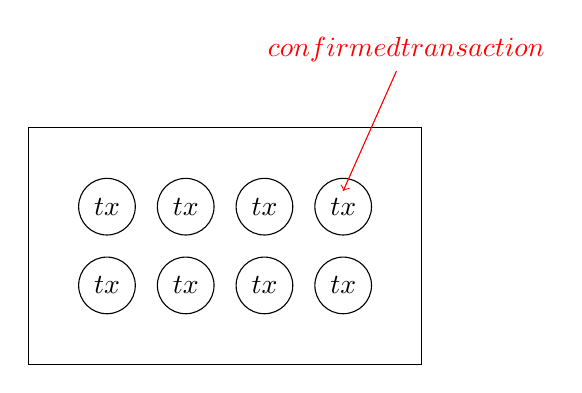
\begin{tikzpicture}
      \draw (0,0) rectangle (5,3);
      \foreach \x in {1,2,...,4}
        \foreach \y in {1,...,2}
          \node[circle,draw, minimum size=0.4cm] at (\x,\y) {$tx$};

      \node[red] (confirm) at (4.8, 4) {$confirmed \text{ }transaction$};
      \draw [->, red] (confirm) -- (4,2.2);
    \end{tikzpicture}
    \caption{A block}
    \label{fig:block:a}
  \end{subfigure}
  \begin{subfigure}[t]{0.50\textwidth}
    \centering
    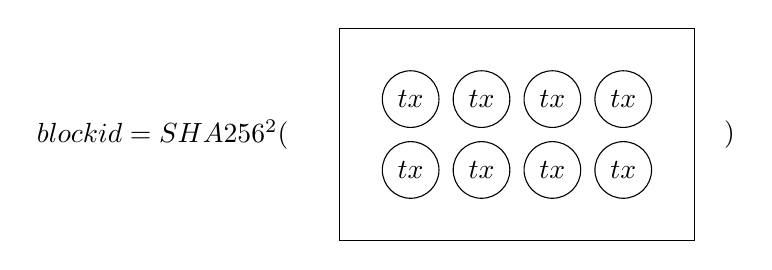
\begin{tikzpicture}[scale=0.9]
      \draw (0,0) rectangle (5,3);
      \foreach \x in {1,2,...,4}
        \foreach \y in {1,...,2}
          \node[circle,draw, minimum size=0.4cm] at (\x,\y) {$tx$};
      \node (txid) at (-2.5,1.5) {$blockid = SHA256^{2}($};
      \node (txid) at (5.5,1.5) {$)$};
    \end{tikzpicture}
    \caption{Bitcoin Block ID}
    \label{fig:block:b}
  \end{subfigure}
  \caption{Blocks}
  \label{fig:blocks}
\end{figure}

\begin{figure}[ht!]
  \centering
  \begin{tikzpicture}
    \foreach \x in {0,1,...,4}
        \pgfmathparse{(\x*3)}
        \edef\position{\pgfmathresult}
        \node[bl_block] (\x) at (\position,0) {$block$};

    \foreach \x in {1,2,...,4}
        \pgfmathparse{(\x-1)}
        \edef\previous{\pgfmathresult}
        \draw [->] (\x) -- (\previous);

  \end{tikzpicture}
  \caption{The blockchain}
  \label{fig:blockchain}
\end{figure}

\begin{figure}[ht!]
  \begin{tikzpicture}
    \foreach \x in {0,1,...,4}{
        \pgfmathparse{(\x*3)}
        \edef\position{\pgfmathresult}
        \node[bl_block] (\x) at (\position,0) {$block$};
        \pgfmathparse{int(\x*10 + 10)}
        \edef\time{\pgfmathresult}
        \node[] at (\position,-2) {$17:\time$};
    }


    \foreach \x in {1,2,...,4}
        \pgfmathparse{(\x-1)}
        \edef\previous{\pgfmathresult}
        \draw [->] (\x) -- (\previous);

    \node[ellipse, draw, red, inner xsep=6ex,inner ysep=3ex] (old_ell) at (0) {};
    \node[ellipse, draw, red, inner xsep=6ex,inner ysep=3ex] (recent_ell) at (4) {};
    \node[red,below=0cm of old_ell] (old) {$oldest\text{ }block\text{ }$};
    \node[red,below=0cm of recent_ell] (recent) {$recent\text{ }block\text{ }$};
  \end{tikzpicture}
  \caption{The blockchain timeline}
  \label{fig:blockchain_timeline}
\end{figure}

\section{Consensus mechanisms}\label{blockchain:consensus_mechanisms}

With the use of the blockchain data structure we manage to have chronological order of the transactions. What remains is a global agreement on order of the blocks among the participants of the network. Someone can easily change the order of two blocks within the chain by changing the respective hashes or producing new ones wherever required~\cite{zindros_thesis}. This would allow an adversary to fake the order of transactions in time, which is an undesired outcome.

The global agreement on a common truth, the global blockchain, is called consensus---a single universal “truth”--- and this is where Bitcoin's novelty is. The consensus mechanism is the core mechanism of the blockchain. Through consensus, the shared state of the ledger comes to an agreement upon a global state, allowing all the nodes of the network to reach the same ledger state. That is, the users of the network agree on a common order of the blocks in the blockchain and therefore on the order of the transactions. Achieving consensus in a distributed system is challenging. A consensus mechanism has to be resilient to node failures, network delays and the existence of malicious nodes.

At high level, every public consensus mechanism works as follows: A ``game'', involving randomness, is taken place where each node of the network participates. The winner of the game is eligible to propose the new block that will be adopted in the blockchain. This is a simple, but marvellous idea. The probabilistic nature of the process is paramount to its security.

There are three basic consensus mechanism categories:

\begin{enumerate}
  \item Proof-of-Work (PoW).
  \item Proof-of-Stake (PoS).
  \item Practical Byzantine Fault Tolerance (PBFT)
\end{enumerate}


\subsection{Proof of Work (PoW)}\label{blockchain:consensus:pow}

A Proof-of-Work (PoW) consensus mechanism, is a consensus mechanism where each node of the network tries to solve a computational puzzle that is computational hard, but feasible to find, and easy to verify correctness. Assuming that hash functions are hard to invert, proof of work usually is established by seeking a range-collision of the hash function on the block~\cite{zindros_thesis}.

\begin{figure}[!ht]
  \centering
  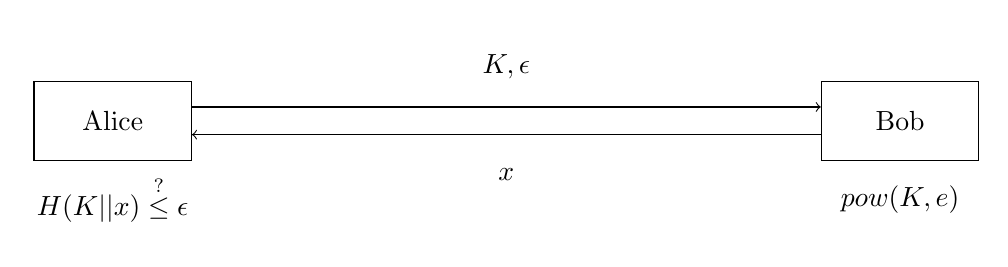
\begin{tikzpicture}[node distance=10cm, minimum height=1cm, minimum width=2cm]
    \node[draw] (a) {Alice};
    \node[draw, right of =a] (b) {Bob};
    \node[below of=a, node distance=1cm] (c) {$H(K || x) \stackrel{?}{\leq} \epsilon$};
    \node[below of=b, node distance=1cm] (d) {$pow(K, e)$};
    \draw[->] ([yshift=0.5em]a.east) -- ([yshift=0.5em]b.west) node[midway, above] {$K, \epsilon$};
    \draw[<-] ([yshift=-0.5em]a.east) -- ([yshift=-0.5em]b.west) node[midway, below] {$x$};
  \end{tikzpicture}
  \caption{The Proof-of-Work protocol}
  \label{fig:consensus:pow}
\end{figure}

Bitcoin~\cite{Zohar:2015:BUH:2817191.2701411} is the first blockchain system that utilizes a PoW for blockchain block generation. It work as follows: A target $\epsilon$ is given and is asked that the hash of the block is smaller than the target. The node can only modify a nonce, which is concatenated with the rest of the block data. By changing the nonce the node can change the block hash. As cryptographic hash functions is assumed to be one-way, the only way to find a hash value smaller than the target is with a series of brute-force trials of different nonce values. Bitcoin's proof-of-work can be summarized as:

\begin{equation*}
  H(txs || nonce || parent\_blockid) \leq \epsilon
\end{equation*}

The network evaluates collectively the target value using a predefined algorithm. That way, the network can control the difficulty of proof-of-work and the expected frequency of block generation is controlled. In Bitcoin the expected rate is one block per 10 minutes.

All the nodes of the network simultaneously try to produce a new block, meaning trying to find a correct nonce satisfying the proof-of-work requirements. Each node monitors the network for blocks and transactions while preparing its block. In its block the node includes all the valid transactions that are not in a previous block and a reference to a parent block. Every node of the network can produce a valid block but each block has to meet the target proof-of-work requirements.

When a hash value less than the target is found by a node, the node gets to add the proposed block to the blockchain and broadcast the new block to to all its neighbours which, in turn, transmit it to the whole network. If a block is found by another node, all the nodes stop the proof of work procedure and start over upon the new block. For a block to be accepted as valid it must contain valid transactions, a valid proof-of-work and a reference to a known valid parent block.

The existence of a transaction in a block makes the transaction valid. The deeper the block is in the blockchain the more difficult is for an adversary to alter the block in which the transaction is confirmed. The reason is, that the time an adversary needs to alter a block grows exponentially in the number of blocks that have followed~\cite{10.1007/978-3-662-46803-6_10}, as she will need to reproduced those blocks and the blockchain is constantly extended. Waiting 6 confirmation blocks to appear after the block in which the transaction is confirmed is enough for a transaction to considered secure.

A PoW system is based on randomness. Each node has a small change to win the block which is approximated proportionally to the computational power of each node. The consensus mechanism depends on having a majority of the miners acting honestly out of self-interest~\cite{antonopoulos2014mastering}.

PoW consensus mechanism works very well in public blockchain systems where trust of the nodes is low eliminating the double-spend problem and guarding against Sybil attacks~\cite{Vu:2009:PCP:1671222}. However, the transaction confirmation time is longer compared to conventional financial services (such as VISA)~\cite{Sompolinsky2015,Zohar:2015:BUH:2817191.2701411,DBLP:journals/corr/abs-1708-05665} resulting in slower transaction confirmation rates. Lastly, the energy waste attributed to the mining process can be very high ---the energy requirements of the Bitcoin protocol are estimated to be comparable to those of a small country~\cite{6912770}.

\begin{lstlisting}[language=C, caption={A simple Proof-of-Work Algorithm}, mathescape=true]
  x = rand();

  do {
    ++x;
  } while (H(K||x) >= $\epsilon$);

  return x;
\end{lstlisting}

\subsection{Proof of Stake (PoS)}\label{blockchain:consensus:pos}

Proof-of-Stake algorithms are designed to overcome the disadvantages of PoW in terms of the high electricity consumption involved in mining~\cite{bl_consensus}
and provide equal security guarantees~\cite{Kiayias2017}. Unlike PoW where the nodes of the network solve computational puzzles in order to create a new block, in PoS the choice
of the block creator among the miners is random, yet relative to the stake the node possesses according to the current blockchain ledger. Maintaining
the blockchain relies on the stakeholders themselves and assigns work to them based on the amount of stake that each possesses as reported in the ledger~\cite{Kiayias2017}. The higher the stake participant, the higher the possibility to be chosen.

Proof-of-Stake algorithms suffer from the so-called “nothing at stake” problem. The “nothing at stake” problem refers to attacks against PoS blockchain systems where shareholders do not have
incentives to follow the protocol and vote simultaneously on multiple blockchains exploiting the fact that little computational effort
is needed to build a PoS blockchain~\cite{Kiayias2017}. Ouroboros is the first provable secure PoS algorithm~\cite{Kiayias2017} and is the main consensus algorithm of the Cardano blockchain~\cite{cardano_site}.

\subsection{Practical Byzantine Fault Tolerance (PBFT)}\label{blockchain:consensus:PBFT}

The Practical Byzantine Fault Tolerance algorithm~\cite{Castro:1999:PBF:296806.296824} is the first practical consensus algorithm with Byzantine Fault Tolerance~\cite{byzantine_fault_tolerance}.
It is based on the concept of state machine replication and replication state voting, and is able to process tens of thousands of requests per second with minimal latency.
The algorithm has only a 3\% overhead over a typical filesystem~\cite{Castro:1999:PBF:296806.296824}.

PBFT and state-machine replication protocols’ downside is related to scalability, in terms of the number of nodes (replicas)~\cite{Vukolić2016} that can be supported.
PBFT has only been scaled and studied up to 20 replicas~\cite{bl_consensus,Vukolić2016}. To overcome this limitation, without compromising security, various PBFT variants,
such as Ripple and Stellar, partition the network into smaller groups called federates and each one runs a local consensus protocol among its members and
global consensus is achieved when certain conditions are being met~\cite{DBLP:journals/corr/abs-1708-05665}.

\begin{table}[!ht]
  \centering
  \begin{tabular}{|l|l|l|l|}
    \hline
    & PoW &	PoS &	PBFT \\ \hline
    Blockchain Type &	Permissionless &	Both &	Permissioned \\ \hline
    Scalability of nodes &	High &	High &	Low \\ \hline
    Scalability of clients &	High &	High &	High \\ \hline
    Transaction rate &	Low &	High &	High \\ \hline
    Latency &	High &	Low &	Minimal \\ \hline
    Power consumption &	High &	Low &	Low \\ \hline
    Token needed &	Yes &	Yes &	No \\ \hline
    Cost of participation &	Yes &	Yes &	No \\ \hline
    Adversary tolerance &	$\leq$ 25\%	& Depends &	$\leq$ 33\% \\ \hline
  \end{tabular}
  \caption{Blockchain consensus mechanisms. Adapted and modified from~\cite{bl_consensus,Vukolić2016}}
  \label{table:blockchain_consensus}
\end{table}

\section{Mining \& incentives}\label{blockchain:mining}

The process of creating a block in a PoW consensus system is known as mining and the participants as miners. The first block was mined by Satoshi Nakamoto~\cite{nakamoto2012bitcoin} and is called the genesis block. Every valid chain starts from the genesis block.

For miners to participate in the network and contribute their computation resources incentives are provided. Normally, in a permissionless blockchains such as Bitcoin or Ethereum a monetary incentive in the form of cryptocurrency incentivize the miners and in a permissioned blockchain finance incentives or access to blockchain data could encourage miners to participate~\cite{deloitte}.

In Bitcoin, the miner is rewarded with a number of bitcoins that are created for the specific block. This happens through a specific type of transaction called \textbf{coinbase}. This type of transaction has an unconnected income edge without a sender and an outcoming edge with recipient the miner that found the particular block. This is how new bitcoin is generated. The amount of coin mined in each block is preagreed on by the network and every four years is reduced by half. Currently, the reward is 12,5 BTC.

\begin{figure}[!ht]
  \centering
  \begin{tikzpicture}
    \node[tx] (A) at (0,0) {$tx$};
    \draw [->] (-3,0) -- (A) node[midway, below]{} node[midway, above]{12.5 BTC};
    \draw [->] (A) -- (3, 0) node[midway, below]{miner} node[midway, above]{12.5 BTC};
  \end{tikzpicture}
  \caption{Coinbase transaction}
  \label{fig:mining:coinbase}
\end{figure}

Another way a miner is rewarded is by collecting transactions fees;  the financial remain of a confirmed transaction. This can happen when a user makes a transaction where the total value of all incoming edges are bigger than the total value of all outcoming edges. In particular the total fees of a block are defined as:

\begin{equation*}
  fees = \sum_{tx \in block} [ \sum_{i \in in(tx) }w(i) -  \sum_{o \in out(tx) }w(o)]
\end{equation*}

\section{Blockchain fork}\label{blockchain:fork}

Due to network latency and the distributed nature of the system, it is possible that two miners will find a block around the same time and some nodes will accept the first block and some others the second one. Both blocks are valid, containing a valid proof of work, valid transactions and both extent the same parent block. In such cases there is a temporary fork in the blockchain, where some nodes are adding blocks to one branch while other nodes are adding blocks to another branch. As a result, two competitive versions of the blockchain will emerge~\cite{antonopoulos2014mastering}. This situation, arise the same problem we have with the transactions: the order of the blocks cannot be defined.

To resolve this, each node always selects the longest brach. At some point, one of the two branches will be extended by a new block. The nodes that were working on the first branch will see that the new branch is the longest and start working immediately on that. Eventually the system will come to an agreement, the longest branch will be accepted and the others will be discarded. The process of chain selection can be likened to voting where mining nodes ``vote'' with their mining power by choosing which chain to extend by mining the next block; the new block itself represents the voting result~\cite{antonopoulos2014mastering}.

\begin{figure}[!ht]
  \centering
  \begin{tikzpicture}
    \foreach \x in {0,1,...,5}
        \pgfmathparse{(\x*2)}
        \edef\position{\pgfmathresult}
        \node[bl_block, minimum width=1cm, fill=blue!30] (\x) at (\position,0) {$block$};

    \foreach \x in {1,2,...,5}
        \pgfmathparse{(\x-1)}
        \edef\previous{\pgfmathresult}
        \draw [->] (\x) -- (\previous);

    \foreach \x in {3,4}
        \pgfmathparse{(\x*2)}
        \edef\position{\pgfmathresult}
        \node[bl_block, minimum width=1cm, fill=orange!30] (\x_fork) at (\position,2) {$block$};

    \draw [->] (4_fork) -- (3_fork);
    \draw [<-] (2.north) -- (3_fork.west);

  \end{tikzpicture}
  \caption{A blockchain fork}
  \label{fig:bl:fork}
\end{figure}

If a malicious adversary wants to do create double spent transactions or execute a denial-of-service, she has to produce a malicious blockchain longer than the honest. To achieve that, an adversary would need to control the majority of the CPU power of the network and specifically the 51\% of the total network’s hashing power. This is called the 51\% attack. It is important to node that this kind of consensus attack affects at best the most recent blocks. Beyond a certain depth blockchain is absolute immutable. In addition, this type of attacks cannot steal or spend coins as the adversary has to forge a signature to produce a valid transaction impersonating another user.

 Bitcoin's security has been formalized and rigorously explored~\cite{10.1007/978-3-662-46803-6_10} over the last years.

\begin{figure}[ht!]
  \centering
  \begin{tikzpicture}
    \foreach \x in {0,1,...,5}
        \pgfmathparse{(\x*2)}
        \edef\position{\pgfmathresult}
        \node[bl_block, minimum width=1cm, fill=blue!30] (\x) at (\position,0) {};

    \foreach \x in {1,2,...,5}
        \pgfmathparse{(\x-1)}
        \edef\previous{\pgfmathresult}
        \draw [->] (\x) -- (\previous);

    \foreach \x in {3,...,6}
        \pgfmathparse{(\x*2)}
        \edef\position{\pgfmathresult}
        \node[bl_block, minimum width=1cm, fill=red!30] (\x_mal) at (\position,2) {};

    \draw [->] (4_mal) -- (3_mal);
    \draw [->] (5_mal) -- (4_mal);
    \draw [->] (6_mal) -- (5_mal);

    \draw [<-] (2.north) -- (3_mal.west);

    \node[circle, draw, minimum size=0.1cm, fill=red] at (4_mal.center) {};
    \node[circle, draw, minimum size=0.1cm, fill=green] at (3.center) {};

    \draw[decorate,decoration={brace,amplitude=10pt, mirror}, xshift=-1.2em, yshift=-1.5em](0, 0) -- (5, 0) node [black,midway,yshift=-1cm, above] {\footnotesize{Honest common prefix}};

    \draw[decorate,decoration={brace,amplitude=10pt, mirror}, xshift=-1.2em, yshift=-1.5em](6, 0) -- (11, 0) node [black,midway,yshift=-1cm, above] {\footnotesize{Honest blockchain}};

    \draw[decorate,decoration={brace,amplitude=10pt}, xshift=-1.2em, yshift=1.5em](6, 2) -- (13, 2) node [black,midway, above, yshift=1em] {\footnotesize{Malicious blockchain}};

  \end{tikzpicture}
  \caption{Double spent attack}
  \label{fig:blockchain:dl_spent}
\end{figure}

\section{Blockchain Types}\label{blockchain:blockchain_types}

There are various types of blockchains varying in restrictions on data access and participation in the consensus process. Each one has its own advantages and disadvantages.

\begin{itemize}
  \item Public Blockchain: A public blockchain is a blockchain, in which there are no restrictions on reading blockchain data -encrypted or not- and validating transactions~\cite{prbc_vs_pubbc}.
  The most common implementation of a public blockchain is Bitcoin~\cite{nakamoto2012bitcoin} and Ethereum~\cite{ethash}.
  \item Federated or Consortium blockchain: In a federated blockchain transaction validation is limited to a predefined list of entities with their identities known to the network. Data access can either be public or restricted~\cite{prbc_vs_pubbc}.
  \item Private blockchain: A private blockchain is a blockchain where consensus mechanism is centralized to one single entity regardless of data access~\cite{prbc_vs_pubbc}.
\end{itemize}

\section{Consensus defined types of Blockchain}\label{blockchain:consensus_blockchain_types}

\begin{itemize}
  \item Permissionless blockchain: A permissionless blockchain is a blockchain, in which there are no restrictions on identities of transaction processors (i.e., users that are eligible to create blocks of transactions)~\cite{prbc_vs_pubbc}.
  \item Permissioned blockchain: A permissioned blockchain is a blockchain, in which transaction processing is performed by a predefined list of subjects with known identities~\cite{prbc_vs_pubbc}.
\end{itemize}

\begin{table}[!ht]
  \centering
  \begin{tabular}{|l|l|l|l|}
    \hline
     & Public & \makecell[cl]{Permissioned \\ (Multiple Entities)} & \makecell[cl]{Private \\ (Single Entity)} \\ \hline
     Participants & \makecell[cl]{Permissionless \\ Anonymous} & \makecell[cl]{Permissioned \\ Identified \\ Trusted} & \makecell[cl]{Permissioned \\ Identified \\ Trusted} \\ \hline
     Data Access & Public & Public or Restricted & Restricted \\ \hline
     Consensus & PoW, PoS & FBTA, PoS & FBTA \\ \hline
  \end{tabular}
  \caption{Blockchain Types. Source~\cite{hub-bl-types}}
  \label{table:blockchain_types}
\end{table}

\section{Blockchain Implementations}\label{blockchain_implementations}

\subsection{Bitcoin}\label{blockchain:impl:bitcoin}

Bitcoin is the first decentralized digital currency. The main currency is called Bitcoin and is used to store and transmit value among participants in the Bitcoin network. The Bitcoin network is a fully distributed peer-to-peer network where anyone can freely join running an open source implementation of the bitcoin protocol and there is no need for trust to the network; in the network any node may be malicious. As a result, Bitcoin is a public permissionless blockchain. Bitcoin's use a Proof-of-Work consensus mechanism for keeping consistent the public ledger, preventing double spend and confirm transactions. Bitcoin is the oldest digital currency decentralized network running from 3 January 2009~\cite{btc_first_block}. As a result, Bitcoin is the most well studied Blockchain network~\cite{10.1007/978-3-662-46803-6_10} with various published papers on different topics such as privacy~\cite{10.1007/978-3-319-70278-0_8, 10.1007/978-3-642-39884-1_2, Bonneau14e.w.:mixcoin, 10.1007/978-3-662-44774-1_9}, economics\cite{Babaioff:2012:BRB:2229012.2229022, 10.1007/978-3-319-70278-0_17, Bentov2017DecentralizedPM, Carlsten:2016:IBW:2976749.2978408}, attacks~\cite{DBLP:journals_corr_Bahack13, DBLP:journals_corr_EyalS13}, network~\cite{10.1007/978-3-662-44774-1_7, 190890} and scalability~\cite{kiayias2017non, 10.1007/978-3-662-53357-4_5, 10.1007/978-3-662-53357-4_8}. Due to the years Bitcoin's blockchain has grow significantly is size making difficult to some devices to store the entire blockchain and run as a full node leading to network centralization. Specifically, as of April 2018 the Bitcoin's blockchain size is over 160GB~\cite{btc_bl_size}.

Bitcoin suffers from scalability due to the limit on the amount of transactions the bitcoin network can process. The transaction processing capacity maximum is estimated between 3.3 and 7 transactions per second~\cite{10.1007/978-3-662-53357-4_8}. The limit is related to the block size limit---the total number of transactions a block can contain--- that was introduces as an anti-spam measure. There are various proposed and activated solutions to address this issue. One activated solution is Segregated Witness (SegWit, BIP 141)~\cite{segwit} which performed as a soft fork and increased the block size by a factor of approximately of two.

As of April 2018, Bitcoin is the most widely used crypto currency~\cite{10.1007/978-3-642-39884-1_2} with over of 100,000 merchants that accept Bitcoin~\cite{btc_merchants} and with the biggest total market cap~\cite{btc_cap}.

\subsection{Ethereum}\label{blockchain:impl:ethereum}

Ethereum is an open-source, public, blockchain-based distributed computing platform featuring smart contract functionality.
It provides a decentralized Turing-complete virtual machine, the Ethereum Virtual Machine (EVM), which can execute scripts using an
international network of public nodes~\cite{ethereum_yellowpaper}. Ethereum provides a cryptocurrency called ether which can be transferred between accounts and gas,
an internal pricing mechanism used to execute contracts and allocate resources on the network. Through EVM, Ethereum provides Solidity a
Turing-complete language for writing smart contracts that enables anyone to build distributed applications making the process much easier and efficient than ever before.
Ethereum use a Proof-of-Work consensus mechanism called Ethash and has been designed to be ASIC-resistant~\cite{ethash}.
Soon Ethereum will be moved to a Proof-of-Stake consensus mechanism called Casper. Ethereum can be implemented as well as a permissioned blockchain~\cite{consortium_chain_development,quorum}.

\subsection{Cardano}\label{blockchain:impl:cardano}

Cardano is a security focused blockchain that utilize the latest research and engineering insights to build a platform suitable for
the highest value applications~\cite{cardano_site}. It supports distributed applications creation and smart contracts verifiable by a method called formal
verification allowing logical proof of correctness of code providing high security. Cardano addresses the need for regulatory oversight while
maintaining consumer privacy and security. Cardano is the first blockchain project to be peer reviewed by academic researchers~\cite{cardano_site} and its consensus
mechanism, Ouroboros, is the first Proof of Stake algorithm to be provably secure~\cite{Kiayias2017}.
Cardano consists of two main layers, one for accounting and one for computation. The accounting layer is called Cardano Settlement Layer (CSL)
and the computation layer Cardano Computation Layer (CCP) where distributed application can be built and run upon. The CCP layer has not been
implemented yet and there is a plan to be released as a beta by the first quarter of 2018~\cite{cardano_parsons}.

\section{Smart Contracts}
\label{smart_contracts}

A smart contract is a computer protocol intended to facilitate, verify, or enforce the negotiation or performance of a contract~\cite{FM548,szabo1996smart}.
The idea of smart contracts proposed in the early 1990s~\cite{FM548}, by Nick Szabo, and have been used primarily in association with cryptocurrencies enabling
parties to formally specify a cryptographically enforceable agreements~\cite{7163021}. A smart contract consists of a set of promises including protocols within which the parties perform on these promises. It can define rules and penalties around an agreement and automatically enforce those obligations. The contractual rules may be partially or fully self-executed, self-enforcing or both. On blockchain technologies a smart contract is any computer program that is executed on blockchain---a general purpose computation.

Bitcoin is the first blockchain that provides a scripting language for expressing simple smart contracts such as ownership of an amount of coins by one or multiple entities. Bitcoin's language is a stack-based scripting language inspired by Forth~\cite{forth_lang} and offers a set of simple serial commands supporting cryptographic primitives such as hash functions and signature verification. The main disadvantage of Bitcoin's language is that is not Turing-complete limiting the type of smart contracts one can create. Furthermore, adding new commands to extent functionality requires either a soft-fork which has to be decided by the majority of bitcoin network or to fork Bitcoin's code and implement a new blockchain supporting the new features in which the Bitcoin's network power is lost. Numerous previous smart contract application atop Bitcoin (e.g., lottery\cite{Andrychowicz:2014:SMC:2650286.2650764,10.1007/978-3-662-44381-1_24},
verifiable computation~\cite{Kumaresan:2014:UBI:2660267.2660380}) have demonstrated the difficulty of Bitcoin's scripting language~\cite{cryptoeprint:2015:675}.

The need of user defined open source blockchain applications emerged. As a result, Ethereum was born which is the first Turing-complete decentralized smart contract framework. In Ethereum, one can create smart contracts in a high level language such as Solidity~\cite{solidity} which in turn is compiled to bytecode that is executable on the Ethereum.

With Ethereum launch, the notion of DApps (decentralized applications) arisen
and a lot of developers and companies are building numerous applications atop Ethereum such as prediction markets~\cite{augur,gnosis}, social media platforms~\cite{akasha,backfeed},
online gambling~\cite{etheroll,coinpoker} and video games~\cite{cryptokitties}. As of January 2018, there are more than 250 live DApps, with hundreds more under development.

\clearpage

\begin{lstlisting}[language=Solidity, caption={An Ethereum Smart Contract}]
pragma solidity ^0.4.16;

contract Namespace{

  struct NameEntry {
      address owner;
  }

  uint32 constant REGISTRATION_COST = 100;
  uint32 constant UPDATE_COST = 10;
  mapping(bytes32 => NameEntry) data;

  function nameNew(bytes32 hash){
      if (msg.value >= REGISTRATION_COST){
          data[hash].owner = msg.sender;
      }
  }

  function nameUpdate(bytes32 name, bytes32 newValue, address newOwner){
      bytes32 hash = sha3(name);
      if (data[hash].owner == msg.sender && msg.value >= UPDATE_COST) {
          data[hash].value = newValue;
          if(newOwner != 0) {
              data[hash].owner = newOwner;
          }
      }
  }

  function nameLookup (bytes32 name) {
      return data[sha3(name)]
  }
}
\end{lstlisting}

\clearpage
